\section{Appendix}\label{sec:Appendix}

\paragraph{Servlet Lifecycle}
Figure~\ref{fig:Server_Servlet} describes the complete lifecycle of a servlet w.r.t. a web server and a web container. The lifecycle steps are described as follows \cite{servlet}:

\begin{figure}[h]
	\centering
	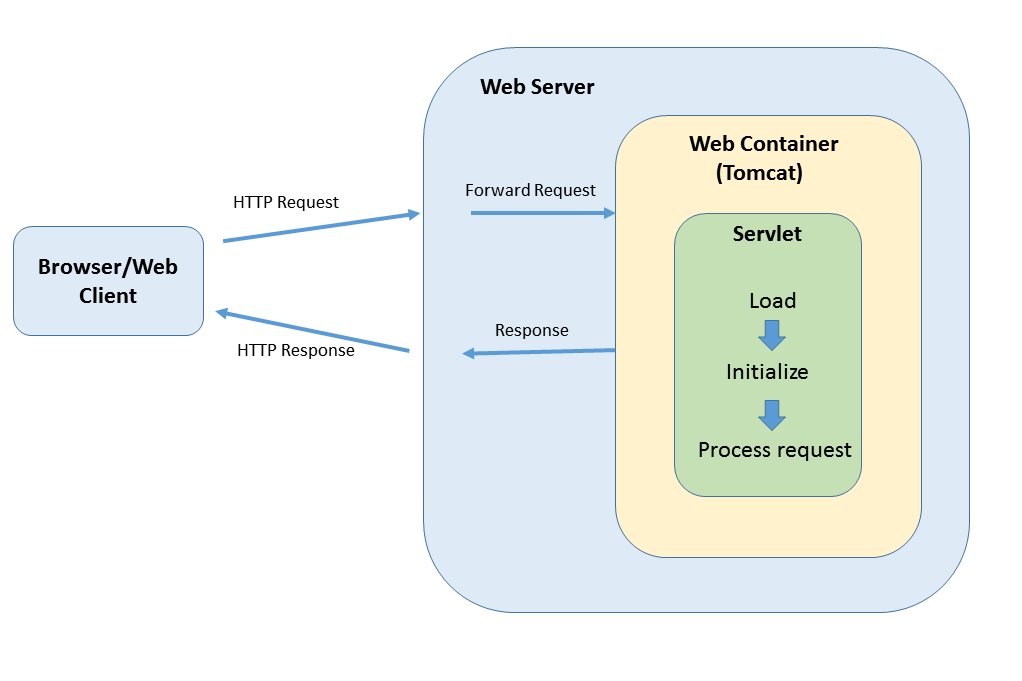
\includegraphics[width=1\textwidth]{figures/Server_Servlet}
	\caption{Servlet Lifecycle}
	\label{fig:Server_Servlet}
\end{figure}

\begin{enumerate}
	\item {The web server receives the \texttt{HTTP request} from the client interacting through a browser. After accepting the request, web server forwards the request to the web container i.e., Tomcat.}
	\item {Web container sends the request to the \texttt{Servlet class}. If an instance of the servlet does not exist, the web container loads the servlet class then creates an instance of the servlet class and initializes the servlet instance by calling the \texttt{init} method.}
	\item {After that, web container invokes the \texttt{service} methods (normally HTTP methods i.e., \texttt{get}, \texttt{post}, \texttt{put}, \texttt{delete}) of the servlet class by passing the request and response objects and the actual processing of the request is done and the response is generated.}
	\item {Web container sends the response to the web server. Afterward, web server creates the HTTP response and send it back to the client.}
\end{enumerate}

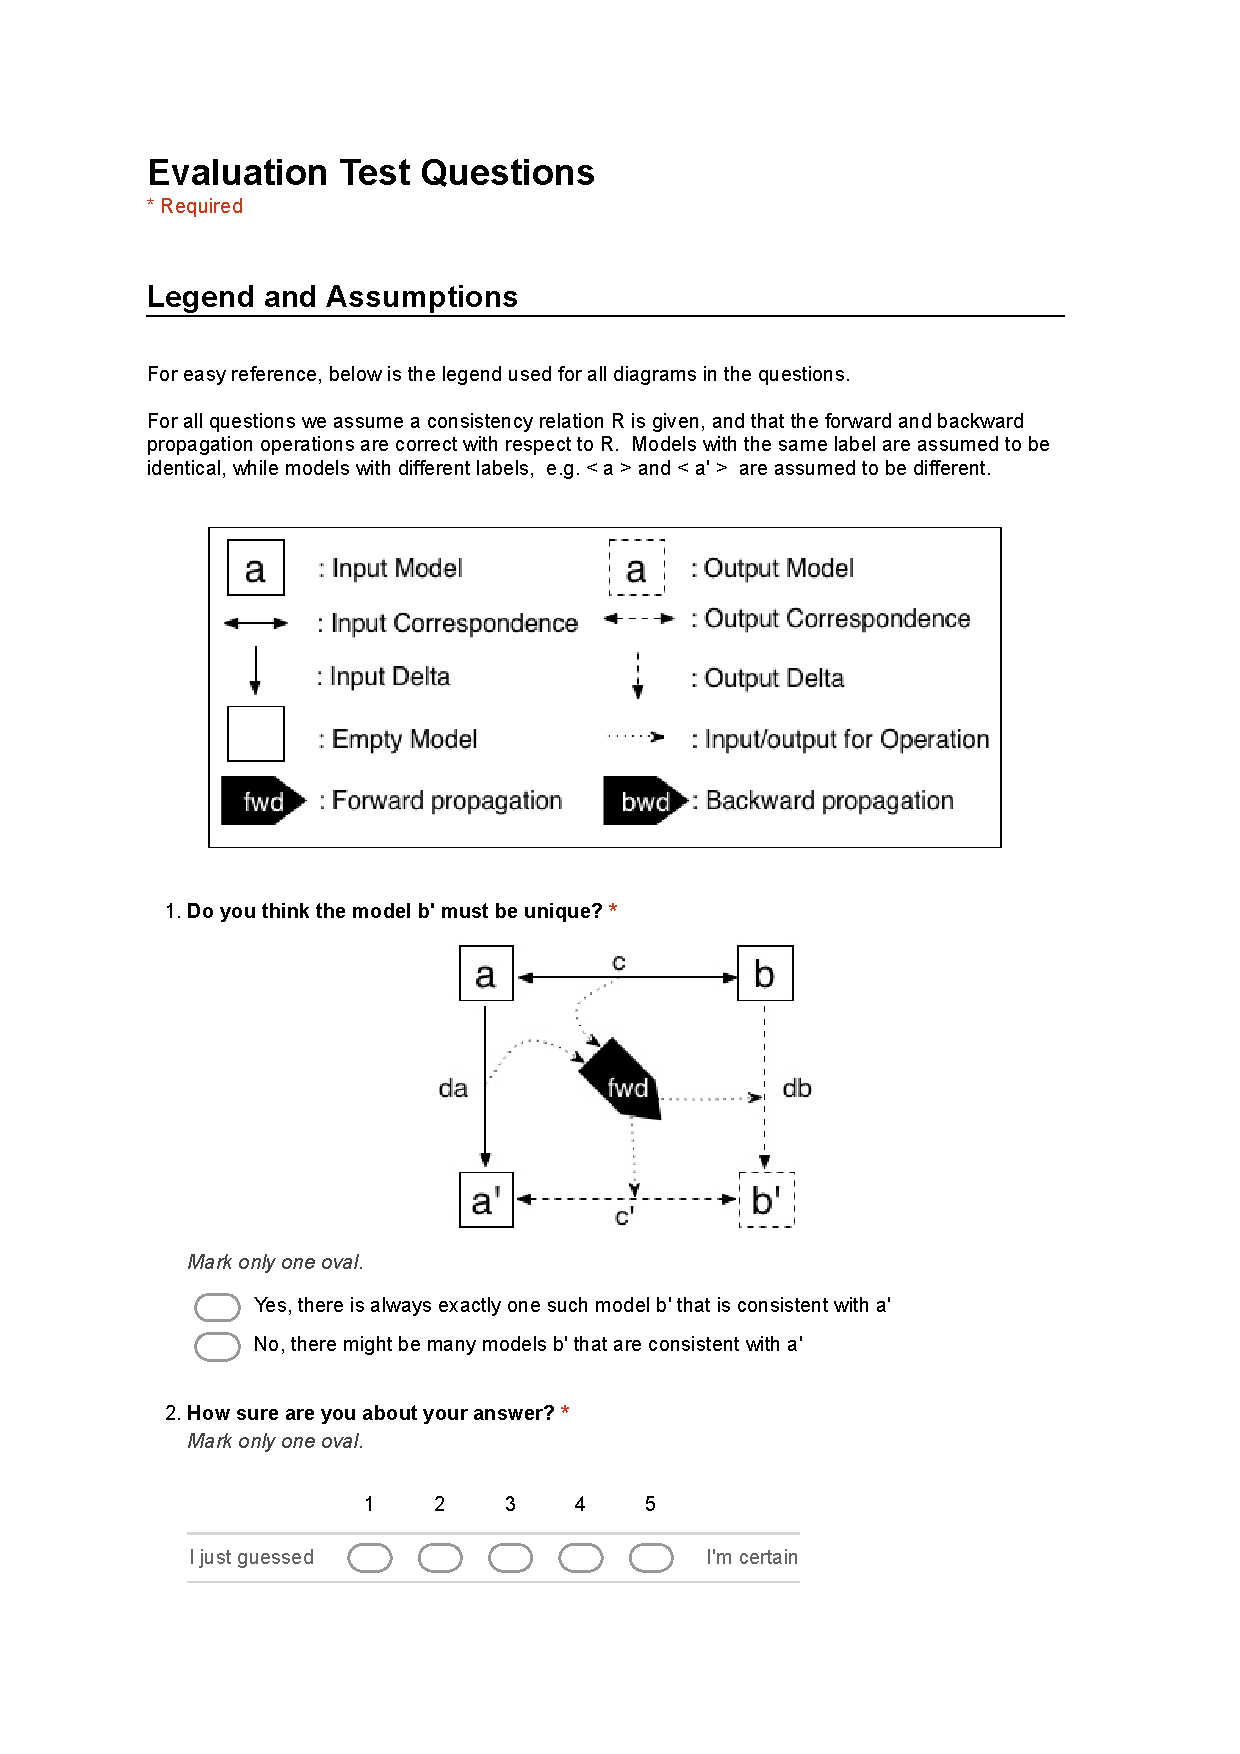
\includepdf[pages={1-5}]{figures/Evaluation_TestQuestions}

\paragraph{Transformation Rules} In this paragraph, I have described all the transformation rules implemented with eMoflon tool for the source and target models. Source models consist of a single \texttt{Grid}, with \texttt{Groups} that can occupy multiple \texttt{Blocks}. \texttt{Blocks} are additionally connected with all their neighboring blocks. Target models consist of a single \texttt{Kitchen} with \texttt{ItemSockets} as placeholders for exactly one \texttt{Item}, i.e., sink, fridge, table etc.

1. \textit{Kitchen\_to\_Grid: }  Figure~\ref{fig:TR_Kitchen_to_Grid} describes that if you create a \texttt{Grid} in the source, then you should create a corresponding \texttt{Kitchen} in the target.

\begin{figure}[h]
	\centering
	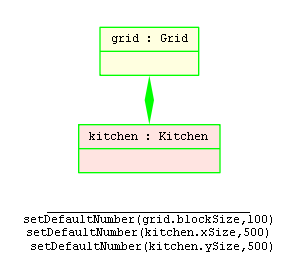
\includegraphics[width=0.7\textwidth]{figures/TR_Kitchen_to_Grid}
	\caption{Transformation Rule: Kitchen\_to\_Grid}
	\label{fig:TR_Kitchen_to_Grid}
\end{figure}

2. \textit{ItemSocket\_to\_Group: } Figure~\ref{fig:TR_ItemSocket_to_Group} describes that if you add a new \texttt{Group} to the grid, then you should add an \texttt{ItemSocket} (a placeholder for items) to the kitchen.

\begin{figure}[h]
	\centering
	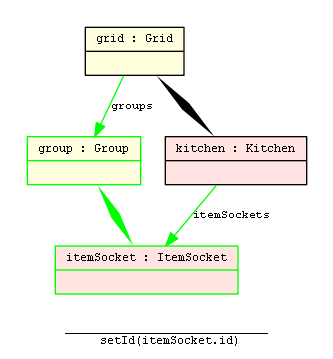
\includegraphics[width=0.5\textwidth]{figures/TR_ItemSocket_to_Group}
	\caption{Transformation Rule: ItemSocket\_to\_Group}
	\label{fig:TR_ItemSocket_to_Group}
\end{figure}

3. \textit{Create\_a\_Sink: } Figure~\ref{fig:TR_Create_a_Sink} describes that a \texttt{Sink} must be created on the western wall and occupies two horizontal blocks.

\begin{figure}[h]
	\centering
	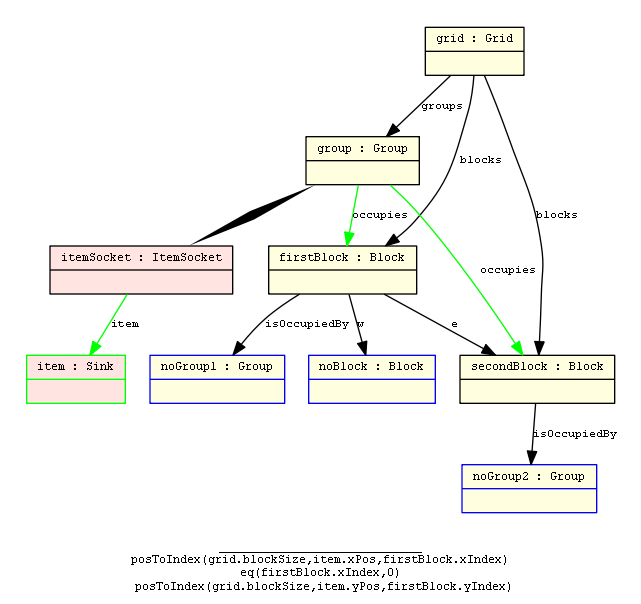
\includegraphics[width=0.7\textwidth]{figures/TR_Create_a_Sink}
	\caption{Transformation Rule: Create\_a\_Sink}
	\label{fig:TR_Create_a_Sink}
\end{figure}

4. \textit{Create\_a\_Fridge: } Figure~\ref{fig:TR_Create_a_Fridge} describes that a \texttt{Fridge} must be created on the northern wall and occupies two vertical blocks.

\begin{figure}[h]
	\centering
	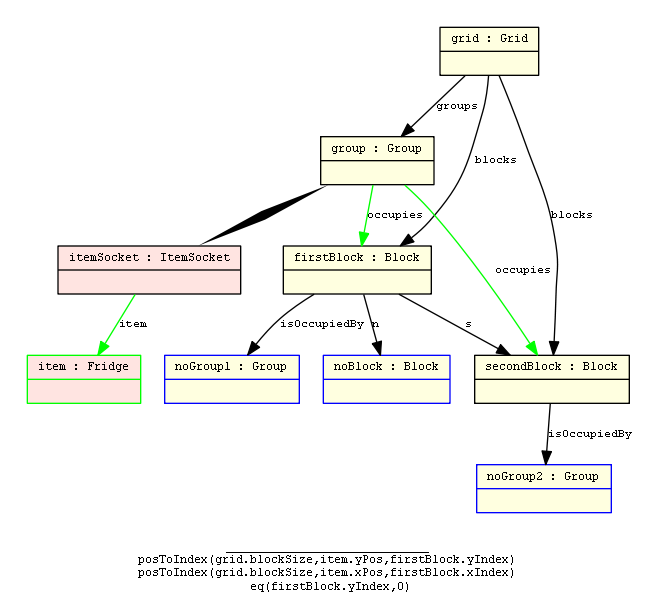
\includegraphics[width=0.8\textwidth]{figures/TR_Create_a_Fridge}
	\caption{Transformation Rule: Create\_a\_Fridge}
	\label{fig:TR_Create_a_Fridge}
\end{figure}

5. \textit{Create\_a\_Horizontal\_Table: } Figure~\ref{fig:TR_Create_a_Horizontal_Table} describes that if you create a \texttt{Horizontal Table}, then its group should be placed on two blocks horizontally.

\begin{figure}[h]
	\centering
	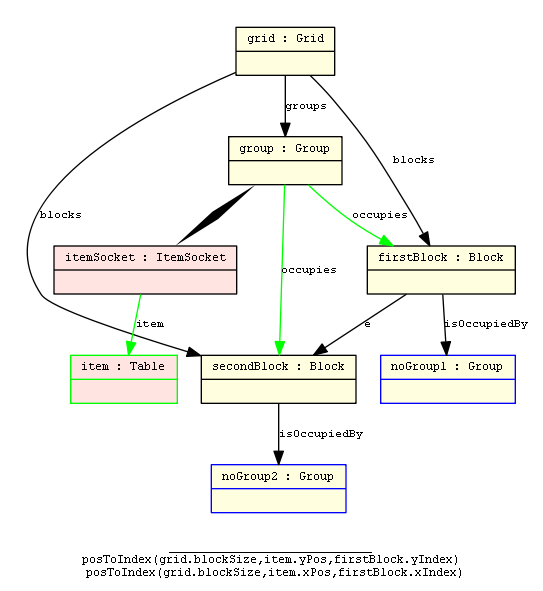
\includegraphics[width=0.8\textwidth]{figures/TR_Create_a_Horizontal_Table}
	\caption{Transformation Rule: Create\_a\_Horizontal\_Table}
	\label{fig:TR_Create_a_Horizontal_Table}
\end{figure}

6. \textit{Create\_a\_Vertical\_Table: } Figure~\ref{fig:TR_Create_a_Vertical_Table} describes that if you create a \texttt{Vertical Table}, then its group should be placed on two blocks vertically.

\begin{figure}[h]
	\centering
	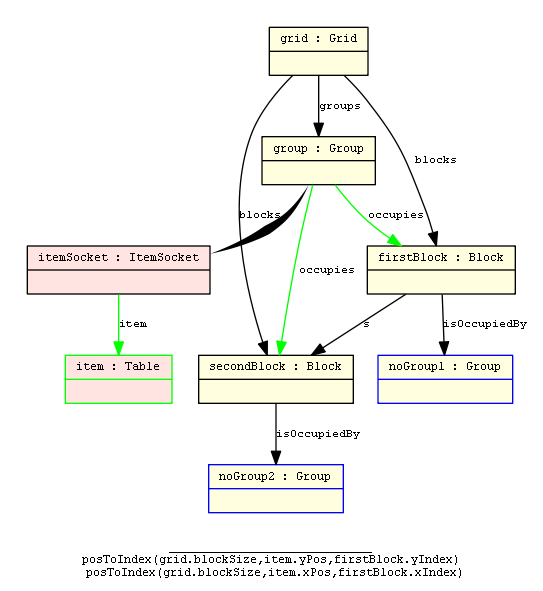
\includegraphics[width=0.8\textwidth]{figures/TR_Create_a_Vertical_Table}
	\caption{Transformation Rule: Create\_a\_Vertical\_Table}
	\label{fig:TR_Create_a_Vertical_Table}
\end{figure}
